\documentclass[twoside]{book}

% Packages required by doxygen
\usepackage{fixltx2e}
\usepackage{calc}
\usepackage{doxygen}
\usepackage[export]{adjustbox} % also loads graphicx
\usepackage{graphicx}
\usepackage[utf8]{inputenc}
\usepackage{makeidx}
\usepackage{multicol}
\usepackage{multirow}
\PassOptionsToPackage{warn}{textcomp}
\usepackage{textcomp}
\usepackage[nointegrals]{wasysym}
\usepackage[table]{xcolor}

% Font selection
\usepackage[T1]{fontenc}
\usepackage[scaled=.90]{helvet}
\usepackage{courier}
\usepackage{amssymb}
\usepackage{sectsty}
\renewcommand{\familydefault}{\sfdefault}
\allsectionsfont{%
  \fontseries{bc}\selectfont%
  \color{darkgray}%
}
\renewcommand{\DoxyLabelFont}{%
  \fontseries{bc}\selectfont%
  \color{darkgray}%
}
\newcommand{\+}{\discretionary{\mbox{\scriptsize$\hookleftarrow$}}{}{}}

% Page & text layout
\usepackage{geometry}
\geometry{%
  a4paper,%
  top=2.5cm,%
  bottom=2.5cm,%
  left=2.5cm,%
  right=2.5cm%
}
\tolerance=750
\hfuzz=15pt
\hbadness=750
\setlength{\emergencystretch}{15pt}
\setlength{\parindent}{0cm}
\setlength{\parskip}{3ex plus 2ex minus 2ex}
\makeatletter
\renewcommand{\paragraph}{%
  \@startsection{paragraph}{4}{0ex}{-1.0ex}{1.0ex}{%
    \normalfont\normalsize\bfseries\SS@parafont%
  }%
}
\renewcommand{\subparagraph}{%
  \@startsection{subparagraph}{5}{0ex}{-1.0ex}{1.0ex}{%
    \normalfont\normalsize\bfseries\SS@subparafont%
  }%
}
\makeatother

% Headers & footers
\usepackage{fancyhdr}
\pagestyle{fancyplain}
\fancyhead[LE]{\fancyplain{}{\bfseries\thepage}}
\fancyhead[CE]{\fancyplain{}{}}
\fancyhead[RE]{\fancyplain{}{\bfseries\leftmark}}
\fancyhead[LO]{\fancyplain{}{\bfseries\rightmark}}
\fancyhead[CO]{\fancyplain{}{}}
\fancyhead[RO]{\fancyplain{}{\bfseries\thepage}}
\fancyfoot[LE]{\fancyplain{}{}}
\fancyfoot[CE]{\fancyplain{}{}}
\fancyfoot[RE]{\fancyplain{}{\bfseries\scriptsize Generated by Doxygen }}
\fancyfoot[LO]{\fancyplain{}{\bfseries\scriptsize Generated by Doxygen }}
\fancyfoot[CO]{\fancyplain{}{}}
\fancyfoot[RO]{\fancyplain{}{}}
\renewcommand{\footrulewidth}{0.4pt}
\renewcommand{\chaptermark}[1]{%
  \markboth{#1}{}%
}
\renewcommand{\sectionmark}[1]{%
  \markright{\thesection\ #1}%
}

% Indices & bibliography
\usepackage{natbib}
\usepackage[titles]{tocloft}
\setcounter{tocdepth}{3}
\setcounter{secnumdepth}{5}
\makeindex

% Hyperlinks (required, but should be loaded last)
\usepackage{ifpdf}
\ifpdf
  \usepackage[pdftex,pagebackref=true]{hyperref}
\else
  \usepackage[ps2pdf,pagebackref=true]{hyperref}
\fi
\hypersetup{%
  colorlinks=true,%
  linkcolor=blue,%
  citecolor=blue,%
  unicode%
}

% Custom commands
\newcommand{\clearemptydoublepage}{%
  \newpage{\pagestyle{empty}\cleardoublepage}%
}

\usepackage{caption}
\captionsetup{labelsep=space,justification=centering,font={bf},singlelinecheck=off,skip=4pt,position=top}

%===== C O N T E N T S =====

\begin{document}

% Titlepage & ToC
\hypersetup{pageanchor=false,
             bookmarksnumbered=true,
             pdfencoding=unicode
            }
\pagenumbering{roman}
\begin{titlepage}
\vspace*{7cm}
\begin{center}%
{\Large My Project }\\
\vspace*{1cm}
{\large Generated by Doxygen 1.8.11}\\
\end{center}
\end{titlepage}
\clearemptydoublepage
\tableofcontents
\clearemptydoublepage
\pagenumbering{arabic}
\hypersetup{pageanchor=true}

%--- Begin generated contents ---
\chapter{Class Index}
\section{Class List}
Here are the classes, structs, unions and interfaces with brief descriptions\+:\begin{DoxyCompactList}
\item\contentsline{section}{\hyperlink{structnode}{node} }{\pageref{structnode}}{}
\item\contentsline{section}{\hyperlink{structnode1}{node1} }{\pageref{structnode1}}{}
\item\contentsline{section}{\hyperlink{structnode__info}{node\+\_\+info} }{\pageref{structnode__info}}{}
\end{DoxyCompactList}

\chapter{File Index}
\section{File List}
Here is a list of all files with brief descriptions\+:\begin{DoxyCompactList}
\item\contentsline{section}{\hyperlink{Lab1_8c}{Lab1.\+c} }{\pageref{Lab1_8c}}{}
\end{DoxyCompactList}

\chapter{Class Documentation}
\hypertarget{classAccount}{}\section{Account Class Reference}
\label{classAccount}\index{Account@{Account}}


{\ttfamily \#include $<$Account.\+h$>$}

\subsection*{Public Member Functions}
\begin{DoxyCompactItemize}
\item 
\hyperlink{classAccount_afde15ac73873bd15583c45db12bde2b3}{Account} (int \hyperlink{classAccount_a92e2552bc9214e93070df37a483fcc1a}{account\+Number}, double \hyperlink{classAccount_a6e41f403b4813738ba835377f212de33}{balance}=0.\+0)
\item 
int \hyperlink{classAccount_aab90becddea7d42ad801ea031c603b80}{get\+Account\+Number} () const 
\item 
double \hyperlink{classAccount_a73bfb6b16b4c29f621e3f3ddc081dc83}{get\+Balance} () const 
\item 
void \hyperlink{classAccount_ac426f0df93883712c99b224645748d67}{set\+Balance} (double \hyperlink{classAccount_a6e41f403b4813738ba835377f212de33}{balance})
\item 
void \hyperlink{classAccount_ab39def1adefa79491042c8a18e4268e0}{credit} (double amount)
\item 
void \hyperlink{classAccount_a3f13036bfe5d033e9664df38724eb2be}{debit} (double amount)
\item 
void \hyperlink{classAccount_a46e741ac1a3b502e3a9411ef9ff1c0a7}{print} () const 
\end{DoxyCompactItemize}
\subsection*{Private Attributes}
\begin{DoxyCompactItemize}
\item 
int \hyperlink{classAccount_a92e2552bc9214e93070df37a483fcc1a}{account\+Number}
\item 
double \hyperlink{classAccount_a6e41f403b4813738ba835377f212de33}{balance}
\end{DoxyCompactItemize}


\subsection{Constructor \& Destructor Documentation}
\index{Account@{Account}!Account@{Account}}
\index{Account@{Account}!Account@{Account}}
\subsubsection[{\texorpdfstring{Account(int account\+Number, double balance=0.\+0)}{Account(int accountNumber, double balance=0.0)}}]{\setlength{\rightskip}{0pt plus 5cm}Account\+::\+Account (
\begin{DoxyParamCaption}
\item[{int}]{account\+Number, }
\item[{double}]{balance = {\ttfamily 0.0}}
\end{DoxyParamCaption}
)}\hypertarget{classAccount_afde15ac73873bd15583c45db12bde2b3}{}\label{classAccount_afde15ac73873bd15583c45db12bde2b3}

\begin{DoxyCode}
8 : \hyperlink{classAccount_a92e2552bc9214e93070df37a483fcc1a}{accountNumber}(no), \hyperlink{classAccount_a6e41f403b4813738ba835377f212de33}{balance}(b) \{ \}
\end{DoxyCode}


\subsection{Member Function Documentation}
\index{Account@{Account}!credit@{credit}}
\index{credit@{credit}!Account@{Account}}
\subsubsection[{\texorpdfstring{credit(double amount)}{credit(double amount)}}]{\setlength{\rightskip}{0pt plus 5cm}void Account\+::credit (
\begin{DoxyParamCaption}
\item[{double}]{amount}
\end{DoxyParamCaption}
)}\hypertarget{classAccount_ab39def1adefa79491042c8a18e4268e0}{}\label{classAccount_ab39def1adefa79491042c8a18e4268e0}

\begin{DoxyCode}
26                                   \{
27    \hyperlink{classAccount_ac426f0df93883712c99b224645748d67}{setBalance}(\hyperlink{classAccount_a6e41f403b4813738ba835377f212de33}{balance}+amount);
28 \}
\end{DoxyCode}


Here is the call graph for this function\+:
\nopagebreak
\begin{figure}[H]
\begin{center}
\leavevmode
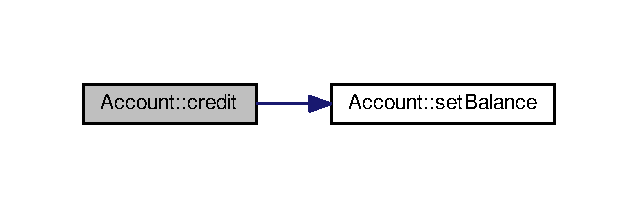
\includegraphics[width=306pt]{classAccount_ab39def1adefa79491042c8a18e4268e0_cgraph}
\end{center}
\end{figure}


\index{Account@{Account}!debit@{debit}}
\index{debit@{debit}!Account@{Account}}
\subsubsection[{\texorpdfstring{debit(double amount)}{debit(double amount)}}]{\setlength{\rightskip}{0pt plus 5cm}void Account\+::debit (
\begin{DoxyParamCaption}
\item[{double}]{amount}
\end{DoxyParamCaption}
)}\hypertarget{classAccount_a3f13036bfe5d033e9664df38724eb2be}{}\label{classAccount_a3f13036bfe5d033e9664df38724eb2be}

\begin{DoxyCode}
31                                  \{
32    \textcolor{keywordflow}{if} (amount <= \hyperlink{classAccount_a6e41f403b4813738ba835377f212de33}{balance}) \{
33       \hyperlink{classAccount_ac426f0df93883712c99b224645748d67}{setBalance}(\hyperlink{classAccount_a6e41f403b4813738ba835377f212de33}{balance}-amount);
34    \} \textcolor{keywordflow}{else} \{
35       cout << \textcolor{stringliteral}{"Amount withdrawn exceeds the current balance!"} << endl;
36    \}
37 \}
\end{DoxyCode}


Here is the call graph for this function\+:
\nopagebreak
\begin{figure}[H]
\begin{center}
\leavevmode
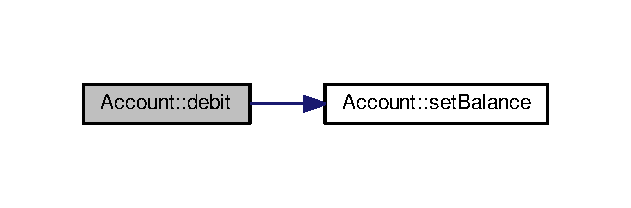
\includegraphics[width=303pt]{classAccount_a3f13036bfe5d033e9664df38724eb2be_cgraph}
\end{center}
\end{figure}


\index{Account@{Account}!get\+Account\+Number@{get\+Account\+Number}}
\index{get\+Account\+Number@{get\+Account\+Number}!Account@{Account}}
\subsubsection[{\texorpdfstring{get\+Account\+Number() const }{getAccountNumber() const }}]{\setlength{\rightskip}{0pt plus 5cm}int Account\+::get\+Account\+Number (
\begin{DoxyParamCaption}
{}
\end{DoxyParamCaption}
) const}\hypertarget{classAccount_aab90becddea7d42ad801ea031c603b80}{}\label{classAccount_aab90becddea7d42ad801ea031c603b80}

\begin{DoxyCode}
11                                     \{
12    \textcolor{keywordflow}{return} \hyperlink{classAccount_a92e2552bc9214e93070df37a483fcc1a}{accountNumber};
13 \}
\end{DoxyCode}
\index{Account@{Account}!get\+Balance@{get\+Balance}}
\index{get\+Balance@{get\+Balance}!Account@{Account}}
\subsubsection[{\texorpdfstring{get\+Balance() const }{getBalance() const }}]{\setlength{\rightskip}{0pt plus 5cm}double Account\+::get\+Balance (
\begin{DoxyParamCaption}
{}
\end{DoxyParamCaption}
) const}\hypertarget{classAccount_a73bfb6b16b4c29f621e3f3ddc081dc83}{}\label{classAccount_a73bfb6b16b4c29f621e3f3ddc081dc83}

\begin{DoxyCode}
16                                  \{
17    \textcolor{keywordflow}{return} \hyperlink{classAccount_a6e41f403b4813738ba835377f212de33}{balance};
18 \}
\end{DoxyCode}
\index{Account@{Account}!print@{print}}
\index{print@{print}!Account@{Account}}
\subsubsection[{\texorpdfstring{print() const }{print() const }}]{\setlength{\rightskip}{0pt plus 5cm}void Account\+::print (
\begin{DoxyParamCaption}
{}
\end{DoxyParamCaption}
) const}\hypertarget{classAccount_a46e741ac1a3b502e3a9411ef9ff1c0a7}{}\label{classAccount_a46e741ac1a3b502e3a9411ef9ff1c0a7}

\begin{DoxyCode}
40                           \{
41    cout << fixed << setprecision(2);
42    cout << \textcolor{stringliteral}{"A/C no: "} << \hyperlink{classAccount_a92e2552bc9214e93070df37a483fcc1a}{accountNumber} << \textcolor{stringliteral}{" Balance=$"} << \hyperlink{classAccount_a6e41f403b4813738ba835377f212de33}{balance} << endl;
43 \}\end{DoxyCode}
\index{Account@{Account}!set\+Balance@{set\+Balance}}
\index{set\+Balance@{set\+Balance}!Account@{Account}}
\subsubsection[{\texorpdfstring{set\+Balance(double balance)}{setBalance(double balance)}}]{\setlength{\rightskip}{0pt plus 5cm}void Account\+::set\+Balance (
\begin{DoxyParamCaption}
\item[{double}]{balance}
\end{DoxyParamCaption}
)}\hypertarget{classAccount_ac426f0df93883712c99b224645748d67}{}\label{classAccount_ac426f0df93883712c99b224645748d67}

\begin{DoxyCode}
21                                  \{
22    \hyperlink{classAccount_a6e41f403b4813738ba835377f212de33}{balance} = b;
23 \}
\end{DoxyCode}


\subsection{Member Data Documentation}
\index{Account@{Account}!account\+Number@{account\+Number}}
\index{account\+Number@{account\+Number}!Account@{Account}}
\subsubsection[{\texorpdfstring{account\+Number}{accountNumber}}]{\setlength{\rightskip}{0pt plus 5cm}int Account\+::account\+Number\hspace{0.3cm}{\ttfamily [private]}}\hypertarget{classAccount_a92e2552bc9214e93070df37a483fcc1a}{}\label{classAccount_a92e2552bc9214e93070df37a483fcc1a}
\index{Account@{Account}!balance@{balance}}
\index{balance@{balance}!Account@{Account}}
\subsubsection[{\texorpdfstring{balance}{balance}}]{\setlength{\rightskip}{0pt plus 5cm}double Account\+::balance\hspace{0.3cm}{\ttfamily [private]}}\hypertarget{classAccount_a6e41f403b4813738ba835377f212de33}{}\label{classAccount_a6e41f403b4813738ba835377f212de33}


The documentation for this class was generated from the following files\+:\begin{DoxyCompactItemize}
\item 
\hyperlink{Account_8h}{Account.\+h}\item 
\hyperlink{Account_8cpp}{Account.\+cpp}\end{DoxyCompactItemize}

\chapter{File Documentation}
\hypertarget{Account_8cpp}{}\section{Account.\+cpp File Reference}
\label{Account_8cpp}\index{Account.\+cpp@{Account.\+cpp}}
{\ttfamily \#include $<$iostream$>$}\\*
{\ttfamily \#include $<$iomanip$>$}\\*
{\ttfamily \#include \char`\"{}Account.\+h\char`\"{}}\\*
Include dependency graph for Account.\+cpp\+:
\nopagebreak
\begin{figure}[H]
\begin{center}
\leavevmode
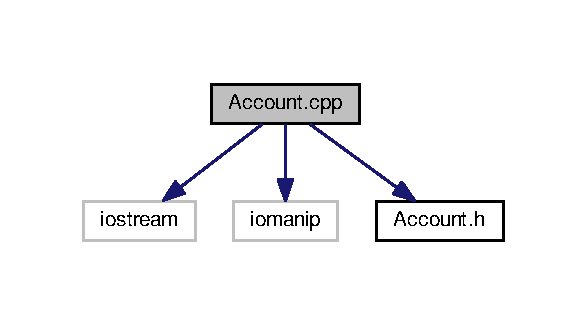
\includegraphics[width=282pt]{Account_8cpp__incl}
\end{center}
\end{figure}

\hypertarget{Account_8h}{}\section{Account.\+h File Reference}
\label{Account_8h}\index{Account.\+h@{Account.\+h}}
This graph shows which files directly or indirectly include this file\+:
\nopagebreak
\begin{figure}[H]
\begin{center}
\leavevmode
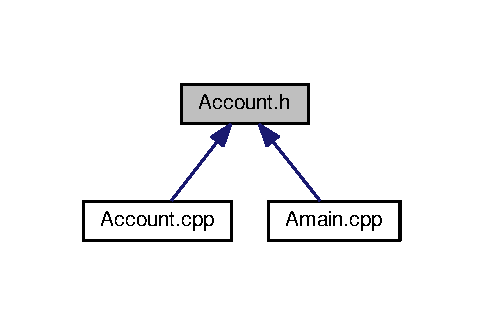
\includegraphics[width=232pt]{Account_8h__dep__incl}
\end{center}
\end{figure}
\subsection*{Classes}
\begin{DoxyCompactItemize}
\item 
class \hyperlink{classAccount}{Account}
\end{DoxyCompactItemize}

\hypertarget{Amain_8cpp}{}\section{Amain.\+cpp File Reference}
\label{Amain_8cpp}\index{Amain.\+cpp@{Amain.\+cpp}}
{\ttfamily \#include $<$iostream$>$}\\*
{\ttfamily \#include \char`\"{}Account.\+h\char`\"{}}\\*
Include dependency graph for Amain.\+cpp\+:
\nopagebreak
\begin{figure}[H]
\begin{center}
\leavevmode
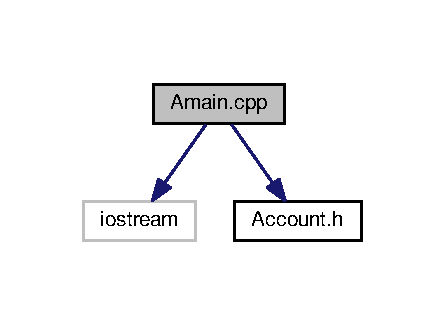
\includegraphics[width=214pt]{Amain_8cpp__incl}
\end{center}
\end{figure}
\subsection*{Functions}
\begin{DoxyCompactItemize}
\item 
int \hyperlink{Amain_8cpp_ae66f6b31b5ad750f1fe042a706a4e3d4}{main} ()
\end{DoxyCompactItemize}


\subsection{Function Documentation}
\index{Amain.\+cpp@{Amain.\+cpp}!main@{main}}
\index{main@{main}!Amain.\+cpp@{Amain.\+cpp}}
\subsubsection[{\texorpdfstring{main()}{main()}}]{\setlength{\rightskip}{0pt plus 5cm}int main (
\begin{DoxyParamCaption}
{}
\end{DoxyParamCaption}
)}\hypertarget{Amain_8cpp_ae66f6b31b5ad750f1fe042a706a4e3d4}{}\label{Amain_8cpp_ae66f6b31b5ad750f1fe042a706a4e3d4}

\begin{DoxyCode}
7            \{
8     \hyperlink{classAccount}{Account} a1(8111, 99.99);
9     a1.print();     \textcolor{comment}{// A/C no: 8111 Balance=$99.99}
10     a1.credit(20);
11     a1.debit(10);
12     a1.print();     \textcolor{comment}{// A/C no: 8111 Balance=$109.99}
13  
14     \hyperlink{classAccount}{Account} a2(8222);  \textcolor{comment}{// default balance}
15     a2.print();        \textcolor{comment}{// A/C no: 8222 Balance=$0.00}
16     a2.setBalance(100);
17     a2.credit(20);
18     a2.debit(200);  \textcolor{comment}{// Amount withdrawn exceeds the current balance!}
19     a2.print();     \textcolor{comment}{// A/C no: 8222 Balance=$120.00}
20     \textcolor{keywordflow}{return} 0;
21 \}\end{DoxyCode}


Here is the call graph for this function\+:
\nopagebreak
\begin{figure}[H]
\begin{center}
\leavevmode
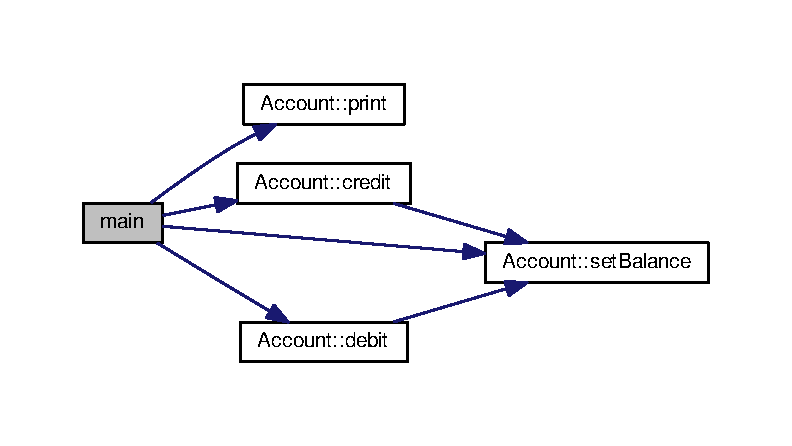
\includegraphics[width=350pt]{Amain_8cpp_ae66f6b31b5ad750f1fe042a706a4e3d4_cgraph}
\end{center}
\end{figure}



%--- End generated contents ---

% Index
\backmatter
\newpage
\phantomsection
\clearemptydoublepage
\addcontentsline{toc}{chapter}{Index}
\printindex

\end{document}
